\documentclass{scrreprt}
\usepackage{listings}
\usepackage{array}
\usepackage{tikz} 
\usepackage{underscore}
\usepackage[bookmarks=true]{hyperref}
\usepackage[utf8]{inputenc}
\usepackage[english]{babel}
\usepackage{enumitem}
\usepackage[a4paper, margin=1in]{geometry}
\usetikzlibrary{shapes, arrows.meta, positioning, backgrounds}
\usetikzlibrary{arrows.meta}
\usetikzlibrary{shapes.geometric, positioning, arrows.meta}
\usetikzlibrary{positioning}
% Define styles for different node types
\tikzstyle{startstop} = [rectangle, rounded corners, minimum width=3cm, minimum height=1cm, text centered, draw=black, fill=red!30]
\tikzstyle{process} = [rectangle, minimum width=3.5cm, minimum height=1cm, text centered, draw=black, fill=blue!30]
\tikzstyle{arrow} = [thick,->,>=stealth]
% Define stickman style
\tikzset{
    startstop/.style={
        rectangle, rounded corners, minimum width=3cm, minimum height=1cm, text centered, draw=black, fill=gray!30
    },
    process/.style={
        rectangle, minimum width=3cm, minimum height=1cm, text centered, draw=black, fill=blue!30
    },
    decision/.style={
        diamond, aspect=2, minimum width=3cm, minimum height=1cm, text centered, draw=black, fill=orange!30
    },
    arrow/.style={
        thick, ->, >=stealth
    },
    stickman/.pic={
        % Head
        \draw[fill=gray] (0,0.6) circle (0.3cm);
        % Body
        \draw[line width=0.5mm] (0,0.3) -- (0,-0.6);
        % Arms
        \draw[line width=0.5mm] (-0.4,0.3) -- (0.4,0.3);
        % Legs
        \draw[line width=0.5mm] (0,-0.6) -- (-0.4,-1.2);
        \draw[line width=0.5mm] (0,-0.6) -- (0.4,-1.2);
}
}
\hypersetup{
    bookmarks=false,    % show bookmarks bar?
    pdftitle={Software Requirement Specification},    % title
    pdfauthor={Jean-Philippe Eisenbarth},                     % author
    pdfsubject={TeX and LaTeX},                        % subject of the document
    pdfkeywords={TeX, LaTeX, graphics, images}, % list of keywords
    colorlinks=true,       % false: boxed links; true: colored links
    linkcolor=blue,       % color of internal links
    citecolor=black,       % color of links to bibliography
    filecolor=black,        % color of file links
    urlcolor=purple,        % color of external links
    linktoc=page            % only page is linked
}
\usetikzlibrary{shapes, arrows.meta, positioning, backgrounds}

\tikzstyle{startstop} = [rectangle, rounded corners, minimum width=3cm, minimum height=1cm, text centered, draw=black, fill=red!30]
\tikzstyle{process} = [rectangle, minimum width=3.5cm, minimum height=1cm, text centered, draw=black, fill=blue!10]
\tikzstyle{database} = [rectangle, minimum width=3cm, minimum height=1cm, text centered, draw=black, fill=orange!30]
\tikzstyle{auth} = [rectangle, minimum width=3cm, minimum height=1cm, text centered, draw=black, fill=green!30]
\tikzstyle{ui} = [rectangle, minimum width=3.5cm, minimum height=1cm, text centered, draw=black, fill=yellow!30]
\tikzstyle{arrow} = [thick,->,>=stealth]



\usepackage{hyperref}
\begin{document}


\begin{center}
    \parbox{0.8\textwidth}{ 
        \centering
        \textbf{Abstract}
    }
\end{center}

The Odyssey Travel website revolutionizes the way individuals plan and experience their journeys, providing a comprehensive platform that caters to all travel needs. Embracing the essence of convenience and personalization, Odyssey Travel offers a diverse range of travel packages, allowing users to effortlessly explore destinations and select their preferred accommodations and transportation options. The platform’s intuitive interface ensures seamless navigation, empowering users to customize their travel plans to match their unique preferences. By bridging the gap between travelers and local service providers, Odyssey Travel promotes cultural exchange and supports local economies. The website not only simplifies the travel booking process but also enhances the overall travel experience by offering tailored recommendations and insights. With a commitment to customer satisfaction and innovation, Odyssey Travel is the ultimate companion for anyone looking to embark on unforgettable adventures.


\tableofcontents

\chapter{Introduction}
In the modern era of digital transformation, travel planning has become increasingly sophisticated, demanding seamless and user-friendly online solutions. This project aims to develop a robust web-based platform for a travel agency, providing an integrated solution for browsing and booking travel packages, transportation, and accommodations. Leveraging cutting-edge technologies like Next.js for efficient front-end rendering, Node.js for scalable server-side operations, SQL for reliable data management, and Tailwind CSS for responsive design, the platform offers a streamlined experience for both visitors and logged-in users. By focusing on ease of use, performance, and security, this project addresses the needs of contemporary travelers, enhancing their journey from planning to booking.

\section{Flow Chart}
The flowchart provides a detailed outline of the steps a user follows on the Odyssey Travel website, from initial interaction to the successful booking of a travel package. It covers user login, registration, browsing of travel packages, booking processes, and the final checkout stage.
\begin{center}
    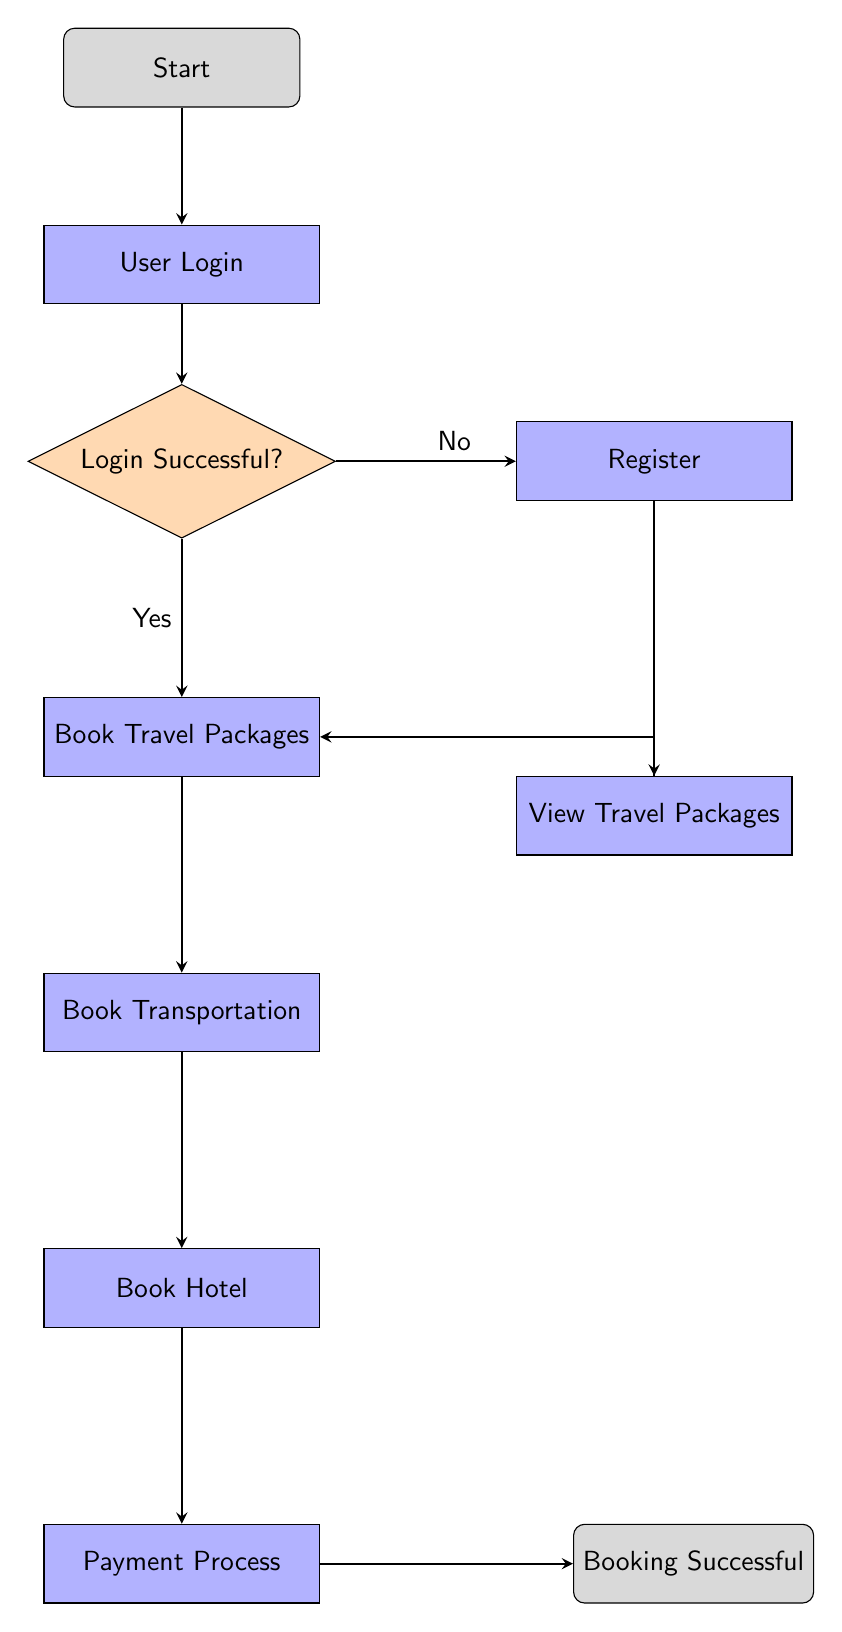
\begin{tikzpicture}[node distance=2cm, every node/.style={fill=white, font=\sffamily, align=center}]
        \tikzstyle{startstop} = [rectangle, rounded corners, minimum width=3cm, minimum height=1cm, text centered, draw=black, fill=gray!30]
        \tikzstyle{process} = [rectangle, minimum width=3.5cm, minimum height=1cm, text centered, draw=black, fill=blue!30]
        \tikzstyle{decision} = [diamond, aspect=2, minimum width=3cm, minimum height=1cm, text centered, draw=black, fill=orange!30]
        \tikzstyle{arrow} = [thick,->,>=stealth]
        \tikzstyle{data} = [trapezium, trapezium left angle=70, trapezium right angle=110, minimum width=3cm, minimum height=1cm, text centered, draw=black, fill=green!30]
    
        % Nodes
        \node (start) [startstop] {Start};
        \node (login) [process, below of=start, yshift=-0.5cm] {User Login};
        \node (checklogin) [decision, below of=login, yshift=-0.5cm] {Login Successful?};
        \node (viewpack) [process, below of=checklogin, yshift=-1.5cm] {Book Travel Packages};
        \node (booktrans) [process, below of=viewpack, yshift=-1.5cm] {Book Transportation};
        \node (bookhotel) [process, below of=booktrans, yshift=-1.5cm] {Book Hotel};
        \node (checkout) [process, below of=bookhotel, yshift=-1.5cm] {Payment Process};
        \node (success) [startstop, right of=checkout, xshift=4.5cm] {Booking Successful};
    
        \node (register) [process, right of=checklogin, xshift=4cm] {Register};
        \node (viewpack2) [process, below of=register, yshift=-2.5cm] {View Travel Packages};
    
        % Connections
        \draw [arrow] (start) -- (login);
        \draw [arrow] (login) -- (checklogin);
        \draw [arrow] (checklogin) -- node[anchor=east] {Yes} (viewpack);
        \draw [arrow] (checklogin.east) -- ++(1.5,0) |- node[anchor=south] {No} (register.west);
        \draw [arrow] (viewpack) -- (booktrans);
        \draw [arrow] (booktrans) -- (bookhotel);
        \draw [arrow] (bookhotel) -- (checkout);
        \draw [arrow] (checkout) -- (success);
    
        \draw [arrow] (register) -- (viewpack2);
        \draw [arrow] (viewpack2) |- (viewpack);
    \end{tikzpicture}
\end{center}
\begin{center}
    \textbf{Fig 1.1: Flow Chart for Travel Agency Software}
\end{center}

\subsection {User Interaction Flow :}
\begin{itemize}
    \item \textbf{Start:} Represents the initial state when a user begins their interaction with the Odyssey Travel website.
    
    \item \textbf{User Login:} The user is prompted to log in to the system by entering their credentials.
    
    \item \textbf{Login Successful?:} A decision point to verify if the user's login credentials are valid.
    \begin{itemize}
        \item \textbf{Yes:} User is authenticated and proceeds to view travel packages.
        \item \textbf{No:} User is redirected to the registration process.
    \end{itemize}
    
    \item \textbf{Register:} For users who are not already registered.
    \begin{itemize}
        \item \textbf{Action:} User completes the registration form with necessary details and submits it.
    \end{itemize}
    
    \item \textbf{View Travel Packages:} Once logged in or registered, the user can browse the available travel packages.
    \begin{itemize}
        \item \textbf{Action:} User explores various travel packages offered by Odyssey Travel.
    \end{itemize}
    
    \item \textbf{View Package Details:} The user selects a travel package to see more detailed information.
    \begin{itemize}
        \item \textbf{Action:} User reviews details such as itinerary, price, inclusions, and exclusions.
    \end{itemize}
    
    \item \textbf{Book Package:} The user decides to book the selected travel package.
    \begin{itemize}
        \item \textbf{Action:} User initiates the booking process for the chosen package.
    \end{itemize}
    
    \item \textbf{Book Transportation:} The user selects and books transportation options related to their travel package.
    \begin{itemize}
        \item \textbf{Action:} User chooses their preferred mode of transportation and confirms the booking.
    \end{itemize}
    
    \item \textbf{Book Hotel:} The user selects and books accommodations as part of the travel package.
    \begin{itemize}
        \item \textbf{Action:} User reviews and selects hotels or lodgings and confirms the booking.
    \end{itemize}
    
    \item \textbf{Add Payment Details:} The user provides payment information to finalize the booking.
    \begin{itemize}
        \item \textbf{Action:} User enters payment details such as credit card information or other payment methods.
    \end{itemize}
    
    \item \textbf{Checkout:} Final review and confirmation of all booking details before completing the transaction.
    \begin{itemize}
        \item \textbf{Action:} User reviews the total cost, verifies all details, and confirms the booking.
    \end{itemize}
    
    \item \textbf{Booking Successful:} Confirmation that the booking has been successfully completed.
    \begin{itemize}
        \item \textbf{Action:} User receives a confirmation email with booking details and further instructions if needed.
    \end{itemize}
\end{itemize}

\chapter{System Architecture}
The system architecture of the Odyssey Travel website is designed to provide a robust and scalable platform for managing travel bookings and related services. It comprises several key components:

\section{System Architecture Diagram}

\begin{figure}[ht]
    \centering
    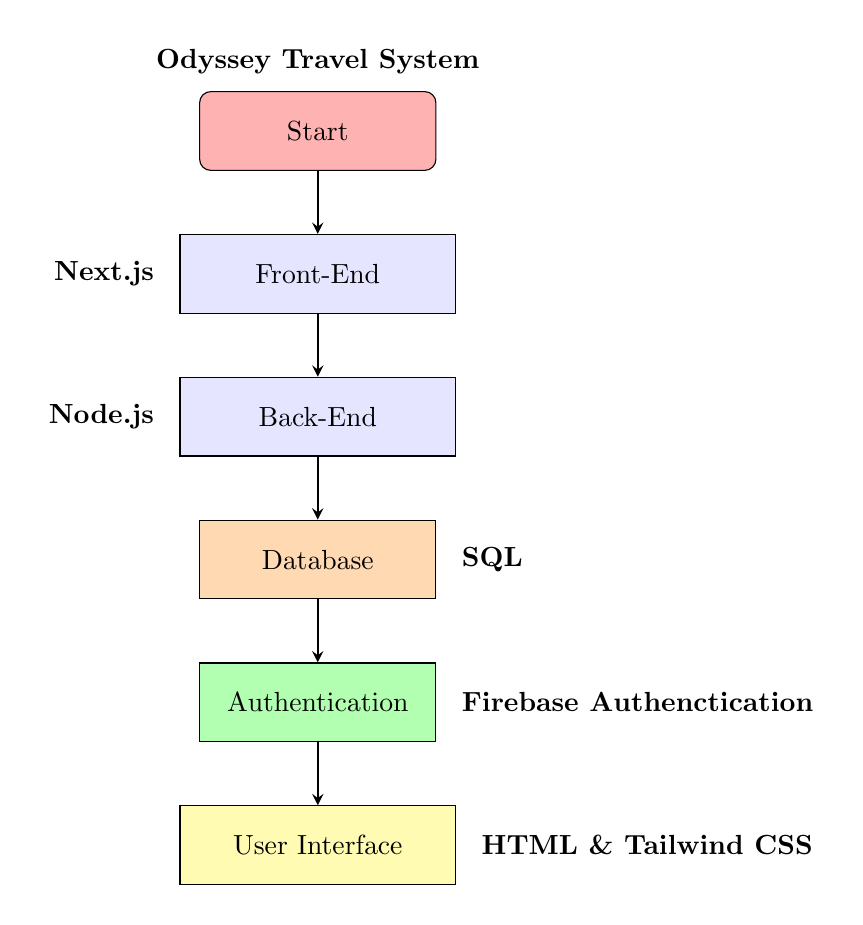
\begin{tikzpicture}[node distance=2cm, background rectangle/.style={fill=white!10}, show background rectangle]
        % Nodes
        \node (start) [startstop] {Start};
        \node (frontend) [process, below=0.8cm of start] {Front-End};
        \node (backend) [process, below=0.8cm of frontend] {Back-End};
        \node (database) [database, below=0.8cm of backend] {Database};
        \node (auth) [auth, below=0.8cm of database] {Authentication};
        \node (ui) [ui, below=0.8cm of auth] {User Interface};
        
        % Arrows
        \draw [arrow] (start) -- (frontend);
        \draw [arrow] (frontend) -- (backend);
        \draw [arrow] (backend) -- (database);
        \draw [arrow] (database) -- (auth);
        \draw [arrow] (auth) -- (ui);
        
        % Labels for nodes
        \node[above=0.1cm of start] {\textbf{Odyssey Travel System}};
        \node[left=0.2cm of frontend] {\textbf{Next.js}};
        \node[left=0.2cm of backend] {\textbf{Node.js}};
        \node[right=0.2cm of database] {\textbf{SQL}};
        \node[right=0.2cm of auth] {\textbf{Firebase Authenctication}};
        \node[right=0.2cm of ui] {\textbf{HTML \& Tailwind CSS}};
        
        % Background color for technology nodes
        \begin{scope}[on background layer]
            \fill[blue!10] (frontend.south west) rectangle (frontend.north east);
            \fill[blue!10] (backend.south west) rectangle (backend.north east);
            \fill[orange!10] (database.south west) rectangle (database.north east);
            \fill[green!10] (auth.south west) rectangle (auth.north east);
            \fill[yellow!10] (ui.south west) rectangle (ui.north east);
        \end{scope}
    \end{tikzpicture}
\end{figure}
\begin{center}
    \textbf{
        Fig 2.1 : System Architecture Diagram}
\end{center}


\begin{table}[ht]
    
\section{System Interaction}
    \centering
    \caption{Front-End}
    \begin{tabular}{|p{4cm}|p{10cm}|}
    \hline
    \textbf{Technology} & Next.js \\
    \hline
    \textbf{Description} & Responsible for rendering the user interface (UI) components of the website. \\
    \hline
    \textbf{Features} &
    \begin{itemize}[label=$\bullet$]
      \item Implements client-side routing
      \item Supports SSR (Server-Side Rendering)
      \item Enables efficient UI updates
    \end{itemize} \\
    \hline
    \end{tabular}
    \end{table}
    
    \vspace{0.5cm}
    
    \begin{table}[ht]
    \centering
    \caption{Back-End}
    \begin{tabular}{|p{4cm}|p{10cm}|}
    \hline
    \textbf{Technology} & Node.js \\
    \hline
    \textbf{Description} & Handles server-side logic, API integrations, and database interactions. \\
    \hline
    \textbf{Features} &
    \begin{itemize}[label=$\bullet$]
      \item Uses Express.js for routing
      \item Integrates with SQL database for data storage and retrieval
    \end{itemize} \\
    \hline
    \end{tabular}
    \end{table}
    
    \vspace{0.5cm}
    
    \begin{table}[ht]
    \centering
    \caption{Database}
    \begin{tabular}{|p{4cm}|p{10cm}|}
    \hline
    \textbf{Technology} & SQL (Structured Query Language) \\
    \hline
    \textbf{Description} & Stores all relevant data including user information, travel packages, bookings, and transaction details. \\
    \hline
    \textbf{Features} &
    \begin{itemize}[label=$\bullet$]
      \item Ensures data integrity
      \item Supports scalability
      \item Allows complex queries for data manipulation
    \end{itemize} \\
    \hline
    \end{tabular}
    \end{table}
    
    \vspace{0.5cm}
    
    \begin{table}[ht]
    \centering
    \caption{Authentication and Authorization}
    \begin{tabular}{|p{4cm}|p{10cm}|}
    \hline
    \textbf{Technology} & Authentication users with Firebase \\
    \hline
    \textbf{Description} & Manages user authentication and authorization processes securely. \\
    \hline
    \textbf{Features} &
    \begin{itemize}[label=$\bullet$]
      \item Implements JWT (JSON Web Tokens) for session management
      \item Ensures secure access to user-specific data and operations
    \end{itemize} \\
    \hline
    \end{tabular}
    \end{table}
    
    \vspace{0.5cm}
    
    \begin{table}[ht]
    \centering
    \caption{User Interface}
    \begin{tabular}{|p{4cm}|p{10cm}|}
    \hline
    \textbf{Technology} & Tailwind CSS \\
    \hline
    \textbf{Description} & Provides a responsive and visually appealing design for the website. \\
    \hline
    \textbf{Features} &
    \begin{itemize}[label=$\bullet$]
      \item Utilizes utility-first CSS framework
      \item Enhances user experience across devices
    \end{itemize} \\
    \hline
    \end{tabular}
    \end{table}
    
    \vspace{0.5cm}
    
    \begin{table}[ht]
    \centering
    \caption{Integration Services}
    \begin{tabular}{|p{4cm}|p{10cm}|}
    \hline
    \textbf{Description} & Facilitates integration with external services such as payment gateways and third-party APIs for real-time data updates and service enhancements. \\
    \hline
    \textbf{Features} &
    \begin{itemize}[label=$\bullet$]
      \item Implements RESTful APIs for seamless communication
    \end{itemize} \\
    \hline
    \end{tabular}
    \end{table}
    
    \begin{table}[ht]
    \centering
    \caption{System Interaction}
    \begin{tabular}{|p{4cm}|p{10cm}|}
    \hline
    \textbf{User Interaction} & Users access the website through a web browser. They interact with the front-end components developed in Next.js, which fetch data from the back-end server via RESTful API endpoints. \\
    \hline
    \textbf{Data Management} & The Node.js server handles incoming requests, processes business logic, and interacts with the SQL database to store and retrieve data related to travel packages, bookings, and user profiles. \\
    \hline
    \textbf{Authentication Flow} & Upon login, the authentication middleware verifies user credentials and issues JWT tokens for subsequent authenticated requests. Unauthorized users are redirected to the registration process. \\
    \hline
    \textbf{Booking Process} & Users navigate through travel packages, select options such as transportation and accommodations, and proceed to book these services. The booking details are stored in the SQL database and confirmed through integration services. \\
    \hline
    \end{tabular}
    \end{table}
    
    \vspace{0.5cm}
    
    
    \begin{table}[ht]
    \section{Scalability and Reliability}
    \centering
    \caption{Scalability and Reliability}
    \begin{tabular}{|p{4cm}|p{10cm}|}
    \hline
    \textbf{Scalability} & Components such as Node.js and SQL database are chosen for their ability to handle increasing loads and data volumes. Horizontal scaling can be achieved by deploying multiple instances of the application and load balancing incoming traffic. \\
    \hline
    \textbf{Reliability} & The use of robust technologies and best practices in authentication, data management, and API integration ensures reliable performance and minimal downtime for users. \\
    \hline
    \end{tabular}
    \end{table}

\chapter{UML}
\section{Activity Diagram}

\section*{Activity Diagram for Travel Agency Software}

The activity diagram illustrates user activities and workflows in the Travel Agency Software, highlighting how users interact with various features.

\begin{itemize}
    \item \textbf{User Initiation:}
    \begin{itemize}
        \item Users start the process as visitors, registered users, or admins.
    \end{itemize}
    \item \textbf{Browsing Packages:}
    \begin{itemize}
        \item Users browse travel packages, viewing details like destination, itinerary, and price.
    \end{itemize}
    \item \textbf{Registration/Login:}
    \begin{itemize}
        \item Users register or log in to access booking and management features.
    \end{itemize}
    \item \textbf{Package Selection and Booking:}
    \begin{itemize}
        \item Registered users select and book travel packages, including dates and options.
    \end{itemize}
    \item \textbf{Applying Coupons:}
    \begin{itemize}
        \item Users apply discount coupons to adjust the package price.
    \end{itemize}
    \item \textbf{Booking Flights and Transportation:}
    \begin{itemize}
        \item Users book flights and transportation linked to their package.
    \end{itemize}
    \item \textbf{Booking Hotels:}
    \begin{itemize}
        \item Users book hotels for their stay based on package details.
    \end{itemize}
    \item \textbf{Admin Management:}
    \begin{itemize}
        \item Admins manage plans, hotels, and tour guides.
    \end{itemize}
    \item \textbf{End Process:}
    \begin{itemize}
        \item Users complete booking or other activities, concluding the process.
    \end{itemize}
\end{itemize}
{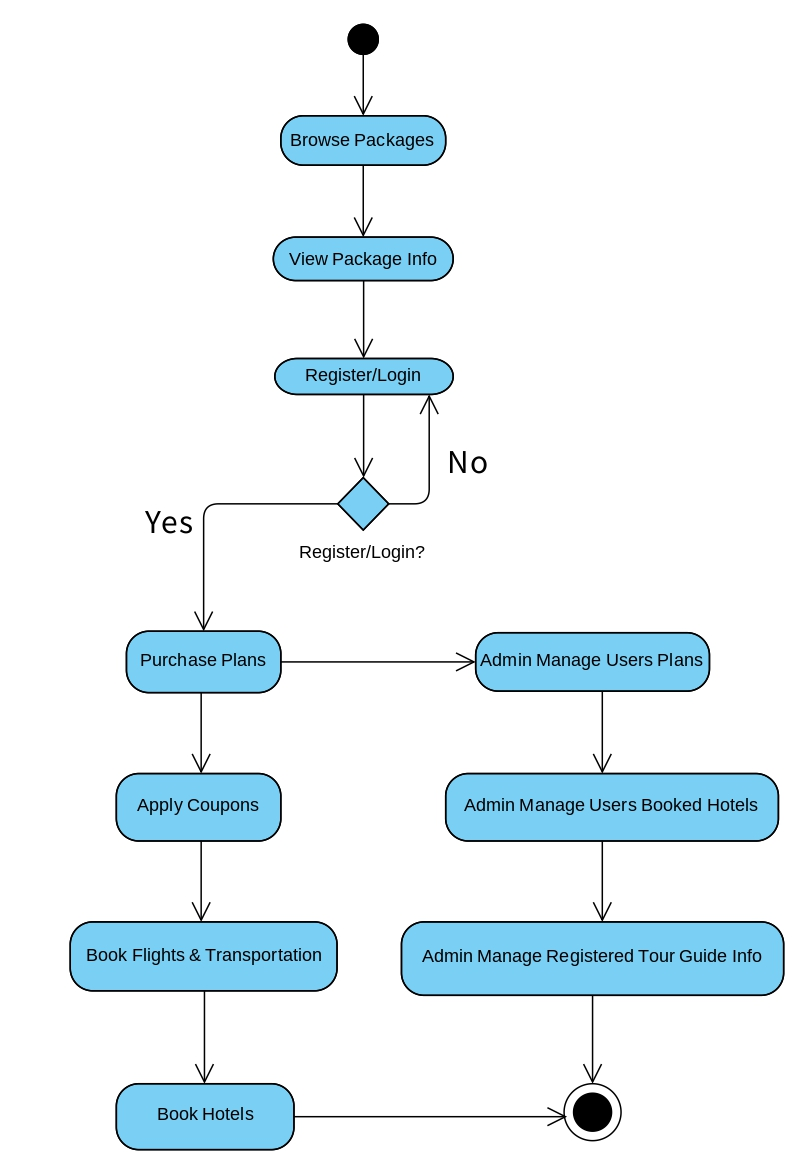
\includegraphics[width=450px, height=500px]{actd.jpg}}

\begin{center}
    \parbox{0.8\textwidth}{ 
        \centering
        \textbf{Figure - 7.9 : Activity Diagram For Travel Agency Software}
    }
\end{center}
\section{Use Cases}
Use Cases help us to identify the actors involved in an interaction and names the type of interaction.
This subsection outlines the Use Cases for our system’s users. Use cases are determined following
the scenarios mentioned in section-6.

\section*{\textbf{7.1.1. UC 1: Users Viewing Packages}}
\textbf{Diagram:}
\newline
\newline
\begin{center}
    \parbox{0.8\textwidth}{ 
        \centering
        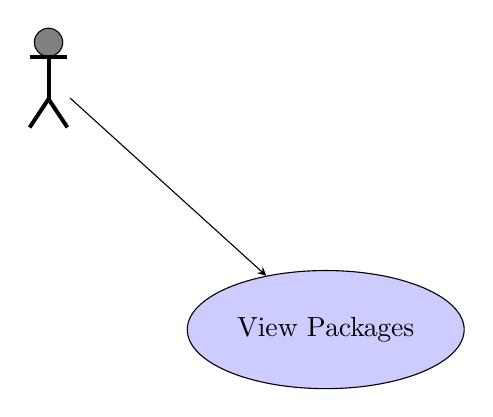
\begin{tikzpicture}[>=stealth]

            % Actor (stickman)
            \node[inner sep=0pt] (user) at (0,0) {\tikz{\pic[scale=0.6] {stickman};}};
        
            % Use Case with color
            \node[ellipse, draw, fill=blue!20, align=center, minimum width=3cm, minimum height=1.5cm, below right=2cm and 2cm of user] (view) {View Packages};
        
            % Relationships
            \draw[->] (user) -- (view);
        
        \end{tikzpicture}
    }
\end{center}

\begin{center}
    \parbox{0.8\textwidth}{ 
        \centering
        \textbf{Figure-7.1: Use Case 01}
    }
\end{center}

\paragraph {\textnormal{Brief Description: 
Users view available travel packages on the Odyssey Travels platform.}}

\textbf{Preconditions:}
\begin{itemize}
    \item User has a working internet connection.
    \item Odyssey Travels application is installed on the device.
\end{itemize}

\textbf{Main Success Scenario:}
\begin{enumerate}
    \item User opens the Odyssey Travels application.
    \item System displays the home screen with navigation options: Home, About, Packages, Login, Signup, Contact Us.
    \item User taps on the "Packages" option from the navigation menu.
    \item System shows the "Packages" page, listing various travel packages available.
    \item User scrolls through the list of packages to explore details and options.
    \item System displays package details including destination, duration, pricing, and amenities.
    \item User selects a specific package for more detailed information.
    \item System shows detailed information such as itinerary, inclusions, and exclusions.
    \item User navigates back to the package list or other sections using navigation buttons.
\end{enumerate}

\textbf{Postcondition:}
\begin{itemize}
    \item System displays the selected package details accurately.
    \item User can proceed to book the selected package or explore other options.
\end{itemize}

\section*{\textbf{7.1.2. UC 2: Purchase Plan}}
\textbf{Diagram:}
\newline
\newline
\begin{center}
    \parbox{0.8\textwidth}{ 
        \centering
        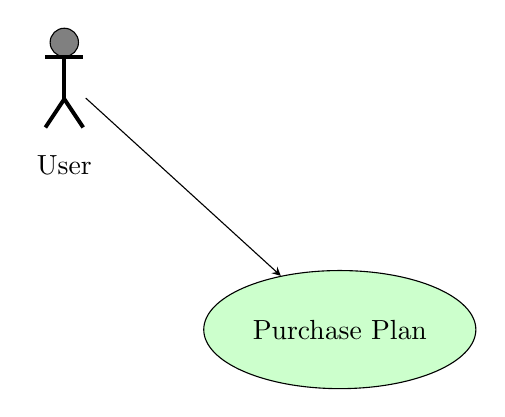
\begin{tikzpicture}[>=stealth]

            % Actor (stickman)
            \node[inner sep=0pt] (user) at (0,0) {\tikz{\pic[scale=0.6] {stickman};}};
            \node[below=0.2cm of user] {User};
        
            % Use Case with color
            \node[ellipse, draw, fill=green!20, align=center, minimum width=3cm, minimum height=1.5cm, below right=2cm and 2cm of user] (purchase) {Purchase Plan};
        
            % Relationships
            \draw[->] (user) -- (purchase);
        
        \end{tikzpicture}
    }
\end{center}

\begin{center}
    \parbox{0.8\textwidth}{ 
        \centering
        \textbf{Figure-7.2: Use Case 02}
    }
\end{center}
\paragraph {\textnormal{Brief Description: 
User selects and purchases a travel plan on the Odyssey Travels platform.\newline
}}
\textbf{Preconditions:}
\begin{itemize}
    \item User has a working internet connection.
    \item Odyssey Travels application is installed on the device.
    \item User is logged into the Odyssey Travels account.
\end{itemize}

\textbf{Main Success Scenario:}
\begin{enumerate}
    \item System displays the home page of the Odyssey Travels application.
    \item User navigates to the "Packages" section from the navigation menu.
    \item System shows a list of available travel packages.
    \item User selects a specific travel package for purchase.
    \item System displays detailed information about the selected package, including itinerary, pricing, and booking options.
    \item User confirms the package selection and taps on the "Book Now" button.
    \item System prompts the user to enter necessary details such as travel dates, number of travelers, and any additional preferences.
    \item User fills in the required information and proceeds to the payment section.
    \item System securely processes the payment using the chosen payment method (e.g., credit card, PayPal).
    \item System confirms the successful booking and displays a confirmation message with booking details.
    \item User receives a confirmation email with the booking details.
\end{enumerate}

\textbf{Postconditions:}
\begin{itemize}
    \item User's selected travel plan is successfully booked and confirmed.
    \item System displays the home page or booking summary for the user to review.
\end{itemize}

\textbf{Alternative Courses:}
\begin{itemize}
    \item[5a.] User explores additional details or options before making a final selection.
    \item[7a.] User adjusts travel details or preferences before confirming the booking.
    \item[9a.] Payment transaction fails or encounters issues; system prompts user to retry or choose an alternative payment method.
\end{itemize}

\textbf{Exceptions:}
\begin{itemize}
    \item User may abandon the booking process at any step before final confirmation.
\end{itemize}

\section*{\textbf{7.1.3. UC 3: Purchase Plan with Apply Coupon}}
\textbf{Diagram:}
\newline
\newline
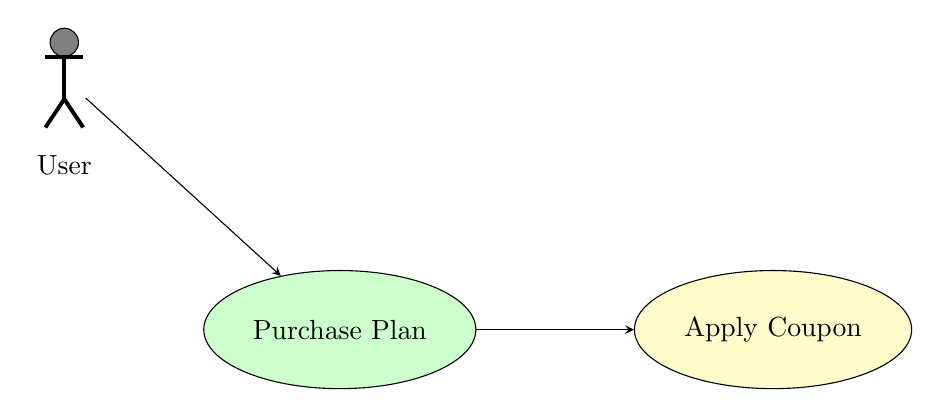
\begin{tikzpicture}[>=stealth]

    % Actor (stickman)
    \node[inner sep=0pt] (user) at (0,0) {\tikz{\pic[scale=0.6] {stickman};}};
    \node[below=0.2cm of user] {User};

    % Use Cases with color
    \node[ellipse, draw, fill=green!20, align=center, minimum width=3cm, minimum height=1.5cm, below right=2cm and 2cm of user] (purchase) {Purchase Plan};
    \node[ellipse, draw, fill=yellow!20, align=center, minimum width=3cm, minimum height=1.5cm, right=2cm of purchase] (apply) {Apply Coupon};

    % Relationships
    \draw[->] (user) -- (purchase);
    \draw[->] (purchase) -- (apply);

\end{tikzpicture}
\begin{center}
    \parbox{0.8\textwidth}{ 
        \centering
        \textbf{Figure-7.3: Use Case 03}
    }
\end{center}


\paragraph {\textnormal{Brief Description: 
User applies a coupon code during the booking process to avail discounts or special offers.}}

\subsection*{\textbf{UC 3: Apply Coupon}}

\textbf{Preconditions:}
\begin{itemize}
    \item User has a working internet connection.
    \item Odyssey Travels application is installed on the device.
    \item User is logged into the Odyssey Travels account.
    \item User has selected a travel package and proceeded to the payment section.
\end{itemize}

\textbf{Main Success Scenario:}
\begin{enumerate}
    \item System displays the booking details and prompts the user to apply a coupon code.
    \item User enters the coupon code in the designated field.
    \item System verifies the coupon validity and applies the discount to the total booking amount.
    \item System updates the payment summary to reflect the discounted price.
    \item User confirms the application of the coupon code.
    \item System confirms the coupon code application and adjusts the total payable amount accordingly.
\end{enumerate}

\textbf{Postconditions:}
\begin{itemize}
    \item System displays the updated booking summary with the discounted price.
    \item User proceeds to complete the booking with the discounted price.
\end{itemize}

\textbf{Alternative Courses:}
\begin{itemize}
    \item[3a.] User enters an invalid coupon code or expired coupon.
    \begin{itemize}
        \item[3a.01.] System displays an error message indicating the issue with the coupon code.
        \item[3a.02.] User can retry with a different coupon code or proceed without applying any coupon.
    \end{itemize}
\end{itemize}

\textbf{Exceptions:}
\begin{itemize}
    \item User may abandon the coupon application process at any step before confirmation.
\end{itemize}


\section*{\textbf{7.1.4. UC 4: Book Flight and Transportation}}


\textbf{Diagram:}
\newline
\newline
\begin{center}
    \parbox{0.8\textwidth}{ 
        \centering
        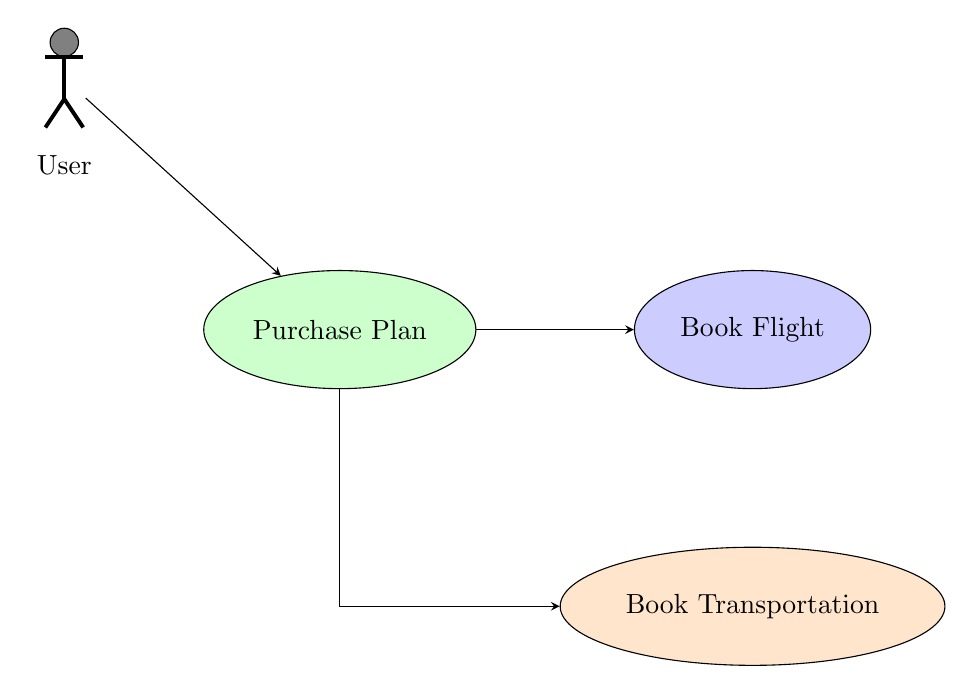
\begin{tikzpicture}[>=stealth]

            % Actor (stickman)
            \node[inner sep=0pt] (user) at (0,0) {\tikz{\pic[scale=0.6] {stickman};}};
            \node[below=0.2cm of user] {User};
        
            % Use Cases with color
            \node[ellipse, draw, fill=green!20, align=center, minimum width=3cm, minimum height=1.5cm, below right=2cm and 2cm of user] (purchase) {Purchase Plan};
            \node[ellipse, draw, fill=blue!20, align=center, minimum width=3cm, minimum height=1.5cm, right=2cm of purchase] (flight) {Book Flight};
            \node[ellipse, draw, fill=orange!20, align=center, minimum width=3cm, minimum height=1.5cm, below=2cm of flight] (transportation) {Book Transportation};
        
            % Relationships
            \draw[->] (user) -- (purchase);
            \draw[->] (purchase) -- (flight);
            \draw[->] (purchase) |- (transportation);
        
        \end{tikzpicture}
    }
\end{center}
\begin{center}
    \parbox{0.8\textwidth}{ 
        \centering
        \textbf{Figure-7.4: Use Case 04}
    }
\end{center}
\paragraph {\textnormal{Brief Description: 
User selects and books flights and transportation services through the Odyssey Travels application.}}


\subsection*{\textbf{UC 4: Book Flight and Transportation}}

\textbf{Preconditions:}
\begin{itemize}
    \item User has a working internet connection.
    \item Odyssey Travels application is installed on the device.
    \item User is logged into the Odyssey Travels account.
    \item User has navigated to the booking section of the app.
\end{itemize}

\textbf{Main Success Scenario:}
\begin{enumerate}
    \item System displays the home page of the Odyssey Travels App.
    \item User taps on the 'Book Flight and Transportation' option from the display screen.
    \item System displays a list of available flights and transportation options.
    \item User selects a flight and transportation option.
    \item System prompts user to enter travel details such as departure date, return date, number of passengers, etc.
    \item User fills in the required details.
    \item System calculates the total fare and displays the payment summary.
    \item User confirms the booking details.
    \item System processes the payment transaction securely.
    \item System confirms the booking with a booking ID and sends a confirmation email or notification to the user.
    \item User receives the booking confirmation and can view the booking details in the app.
\end{enumerate}

\textbf{Postconditions:}
\begin{itemize}
    \item System updates the user's booking history with the new booking details.
    \item User can access the booked flight and transportation details under their account.
\end{itemize}

\textbf{Alternative Courses:}
\begin{itemize}
    \item[5a.] User searches for a specific flight or transportation option not listed.
    \begin{itemize}
        \item[5a.01.] System displays a message indicating no results found.
        \item[5a.02.] User can retry with different search criteria or contact support.
    \end{itemize}
\end{itemize}

\textbf{Exceptions:}
\begin{itemize}
    \item User may abandon the booking process at any step before confirming the payment.
\end{itemize}



\section*{\textbf{7.1.5. UC 5: Book Hotel}}


\textbf{Diagram:}
\newline
\newline
\begin{center}
    \parbox{0.8\textwidth}{ 
        \centering
        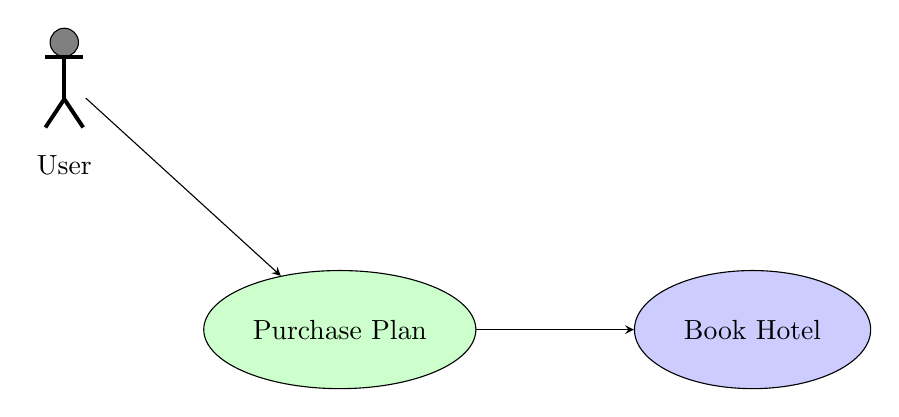
\begin{tikzpicture}[>=stealth]

            % Actor (stickman)
            \node[inner sep=0pt] (user) at (0,0) {\tikz{\pic[scale=0.6] {stickman};}};
            \node[below=0.2cm of user] {User};
        
            % Use Cases with color
            \node[ellipse, draw, fill=green!20, align=center, minimum width=3cm, minimum height=1.5cm, below right=2cm and 2cm of user] (purchase) {Purchase Plan};
            \node[ellipse, draw, fill=blue!20, align=center, minimum width=3cm, minimum height=1.5cm, right=2cm of purchase] (hotel) {Book Hotel};
        
            % Relationships
            \draw[->] (user) -- (purchase);
            \draw[->] (purchase) -- (hotel);
        
        \end{tikzpicture}
    }
\end{center}
\begin{center}
    \parbox{0.8\textwidth}{ 
        \centering
        \textbf{Figure-7.5: Use Case 05}
    }
\end{center}

\paragraph {\textnormal{Brief Description: 
User selects and books accommodations through the Odyssey Travels application.}}


\subsection*{\textbf{UC 5: Book Hotel}}

\textbf{Preconditions:}
\begin{itemize}
    \item User has a working internet connection.
    \item Odyssey Travels application is installed on the device.
    \item User is logged into the Odyssey Travels account.
    \item User has navigated to the hotel booking section of the app.
\end{itemize}

\textbf{Main Success Scenario:}
\begin{enumerate}
    \item System displays the home page of the Odyssey Travels App.
    \item User taps on the 'Book Hotel' option from the display screen.
    \item System displays a list of available hotels based on the user's search criteria.
    \item User selects a hotel from the list.
    \item System prompts user to enter details such as check-in date, check-out date, number of rooms, etc.
    \item User fills in the required details.
    \item System calculates the total cost and displays the payment summary.
    \item User confirms the booking details.
    \item System processes the payment transaction securely.
    \item System confirms the hotel booking with a booking ID and sends a confirmation email or notification to the user.
    \item User receives the booking confirmation and can view the booking details in the app.
\end{enumerate}

\textbf{Postconditions:}
\begin{itemize}
    \item System updates the user's booking history with the new hotel booking details.
    \item User can access the booked hotel details under their account.
\end{itemize}

\textbf{Alternative Courses:}
\begin{itemize}
    \item[5a.] User searches for a specific hotel not listed.
    \begin{itemize}
        \item[5a.01.] System displays a message indicating no results found.
        \item[5a.02.] User can retry with different search criteria or contact support.
    \end{itemize}
\end{itemize}

\textbf{Exceptions:}
\begin{itemize}
    \item User may abandon the booking process at any step before confirming the payment.
\end{itemize}


\section*{\textbf{7.1.6. UC 6: Admin View and Accept/Delete Plans}}
\textbf{Diagram:}
\newline
\newline

\begin{center}
    \parbox{0.8\textwidth}{ 
        \centering
       
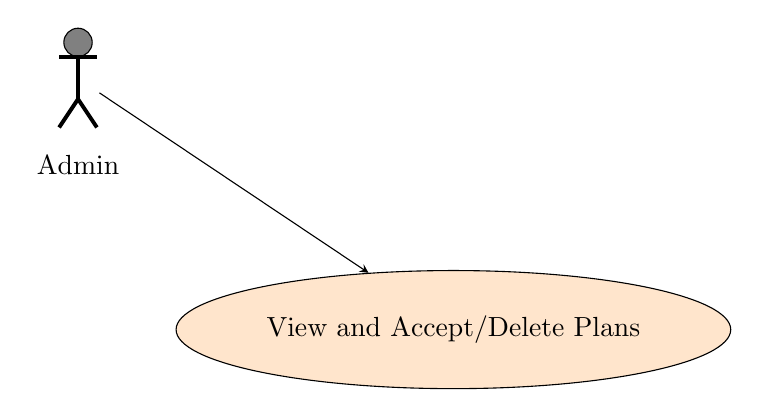
\begin{tikzpicture}[>=stealth]

    % Actor (Admin)
    \node[inner sep=0pt] (admin) at (0,0) {\tikz{\pic[scale=0.6] {stickman};}};
    \node[below=0.2cm of admin] {Admin};

    % Use Case with color
    \node[ellipse, draw, fill=orange!20, align=center, minimum width=4cm, minimum height=1.5cm, below right=2cm and 2cm of admin] (view) {View and Accept/Delete Plans};

    % Relationships
    \draw[->] (admin) -- (view);

\end{tikzpicture}
    }
\end{center}
\begin{center}
    \parbox{0.8\textwidth}{ 
        \centering
        \textbf{Figure-7.6: Use Case 06}
    }
\end{center}

\paragraph {\textnormal{Brief Description: 
Admin reviews and manages travel plans submitted by users, either accepting or deleting them based on predefined criteria.}}


\subsection*{\textbf{Main Success Scenario:}}

\begin{enumerate}
    \item \textbf{Admin logs into the Odyssey Travels admin panel.}
    \item Navigates to "Manage Travel Plans" section.
    \item Views list of submitted plans.
    \item Selects a plan for detailed review.
    \item Reviews plan details (itinerary, user info, pricing).
    \item Evaluates plan against criteria.
    \item Accepts plan: updates status, notifies user.
    \item Deletes plan: removes from system, notifies user.
    \item Records decision and notes.
\end{enumerate}

\subsection*{\textbf{Postconditions:}}

\begin{itemize}
    \item Plan status updated in database.
    \item User notified of plan status.
\end{itemize}

\subsection*{\textbf{Alternative Courses:}}

\begin{itemize}
    \item Requests additional info or corrections from user.
    \item Communicates via internal messaging or email.
\end{itemize}

\subsection*{\textbf{Exceptions:}}

\begin{itemize}
    \item Technical issues hindering plan access.
    \item Admin postpones review.
\end{itemize}

\section*{\textbf{7.1.7. UC 7: Admin View and Edit Booked Hotels of Users}}
\textbf{Diagram:}
\newline
\newline

\begin{center}
    \parbox{0.8\textwidth}{ 
        \centering
        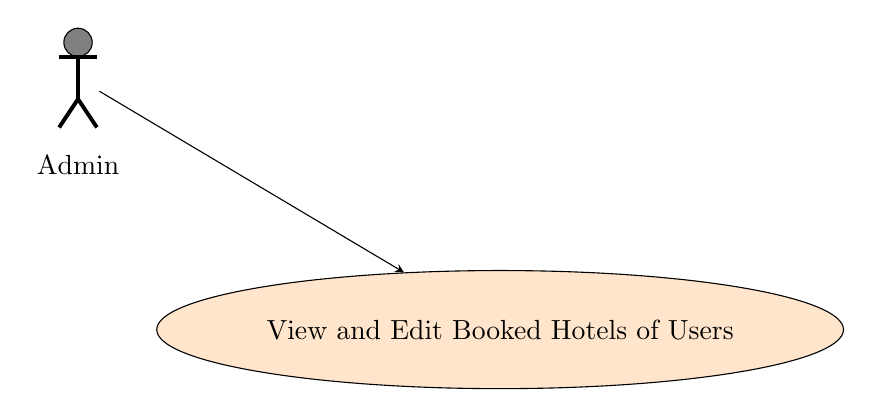
\begin{tikzpicture}[>=stealth]
            % Actor (Admin)
            \node[inner sep=0pt] (admin) at (0,0) {\tikz{\pic[scale=0.6] {stickman};}};
            \node[below=0.2cm of admin] {Admin};
        
            % Use Case with color
            \node[ellipse, draw, fill=orange!20, align=center, minimum width=6cm, minimum height=1.5cm, below right=2cm and 2cm of admin] (view) {View and Edit Booked Hotels of Users};
        
            % Relationships
            \draw[->] (admin) -- (view);
        
        \end{tikzpicture}
    }
\end{center}
\begin{center}
    \parbox{0.8\textwidth}{ 
        \centering
        \textbf{Figure-7.7: Use Case 07}
    }
\end{center}

\paragraph {\textnormal{Brief Description: 
Admin accesses and modifies hotel bookings made by users through the Odyssey Travels platform.}}

\subsection*{\textbf{Main Success Scenario:}}

\begin{enumerate}
    \item Admin logs into the Odyssey Travels admin dashboard.
    \item Navigates to "Manage Booked Hotels" section.
    \item Views list of booked hotels with user details.
    \item Selects a booked hotel for editing.
    \item Reviews booking details (dates, rooms, preferences).
    \item Edits booking information as required.
    \item Confirms changes and updates the booking.
    \item Notifies user of any modifications.
\end{enumerate}

\subsection*{\textbf{Postconditions:}}

\begin{itemize}
    \item Booking details updated in the system.
    \item User notified of changes made.
\end{itemize}

\subsection*{\textbf{Alternative Courses:}}

\begin{itemize}
    \item Requests additional information or clarifications from the user.
    \item Provides support or resolves issues related to the booking.
\end{itemize}

\subsection*{\textbf{Exceptions:}}

\begin{itemize}
    \item System downtime affecting access to bookings.
    \item Admin defers editing due to unforeseen circumstances.
\end{itemize}

\section*{\textbf{7.1.8. UC 8: Admin View, Edit, Delete Registered Tour Guide's Information}}
\textbf{Diagram:}
\newline

\begin{center}
    \parbox{0.8\textwidth}{ 
        \centering
        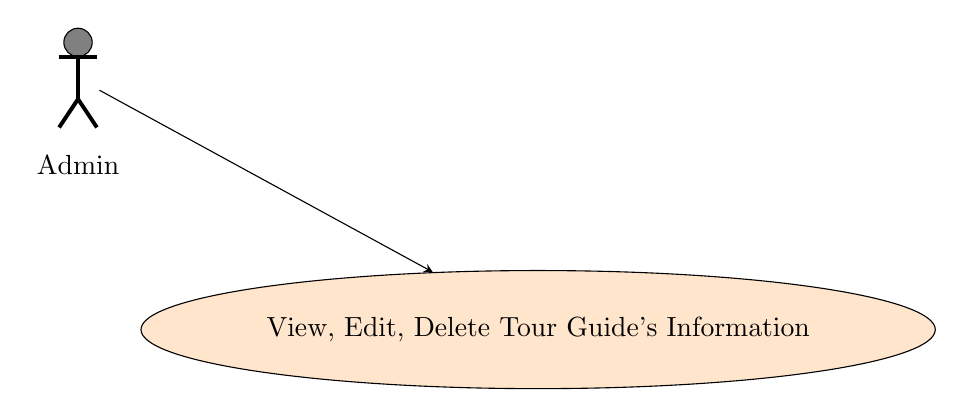
\begin{tikzpicture}[>=stealth]

            % Actor (Admin)
            \node[inner sep=0pt] (admin) at (0,0) {\tikz{\pic[scale=0.6] {stickman};}};
            \node[below=0.2cm of admin] {Admin};
        
            % Use Case with color
            \node[ellipse, draw, fill=orange!20, align=center, minimum width=6cm, minimum height=1.5cm, below right=2cm and 2cm of admin] (view) {View, Edit, Delete Tour Guide's Information};
        
            % Relationships
            \draw[->] (admin) -- (view);
        
        \end{tikzpicture}
    }
\end{center}
\begin{center}
    \parbox{0.8\textwidth}{ 
        \centering
        \textbf{Figure-7.8: Use Case 08}
    }
\end{center}

\paragraph {\textnormal{Brief Description: 
Admin manages the information of registered tour guides within the Odyssey Travels platform.}}

\subsection*{\textbf{Main Success Scenario:}}

\begin{enumerate}
    \item Admin logs into the Odyssey Travels admin dashboard.
    \item Navigates to "Manage Tour Guides" section.
    \item Views list of registered tour guides with their details.
    \item Selects a tour guide for viewing or editing.
    \item Reviews tour guide's information (contact details, certifications).
    \item Edits tour guide's information as required.
    \item Confirms changes and updates the tour guide's profile.
    \item Deletes tour guide's profile if necessary, after confirmation.
\end{enumerate}

\subsection*{\textbf{Postconditions:}}

\begin{itemize}
    \item Tour guide's information updated or deleted as per admin's actions.
    \item System reflects changes immediately.
\end{itemize}

\subsection*{\textbf{Alternative Courses:}}

\begin{itemize}
    \item Admin requests additional documentation or updates from the tour guide.
    \item Provides feedback or support regarding certification requirements.
\end{itemize}

\subsection*{\textbf{Exceptions:}}

\begin{itemize}
    \item Technical issues or system errors may delay updates.
    \item Admin decides to defer deletion due to ongoing bookings or other dependencies.
\end{itemize}

\section{Use Case Diagram}

A use case diagram is pivotal in illustrating a user's engagements with the system, depicting the correlation between the user and various use cases they engage in. This diagram serves to provide a comprehensive overview of the system and supports the detailed design process. The UML use case diagram comprises a collection of use cases that encompass all conceivable interactions outlined in the system requirements (Section 6). The use case diagram for Odyssey Travels is delineated in Figure-7.1.

\subsection *{ Use Case Diagram : }
{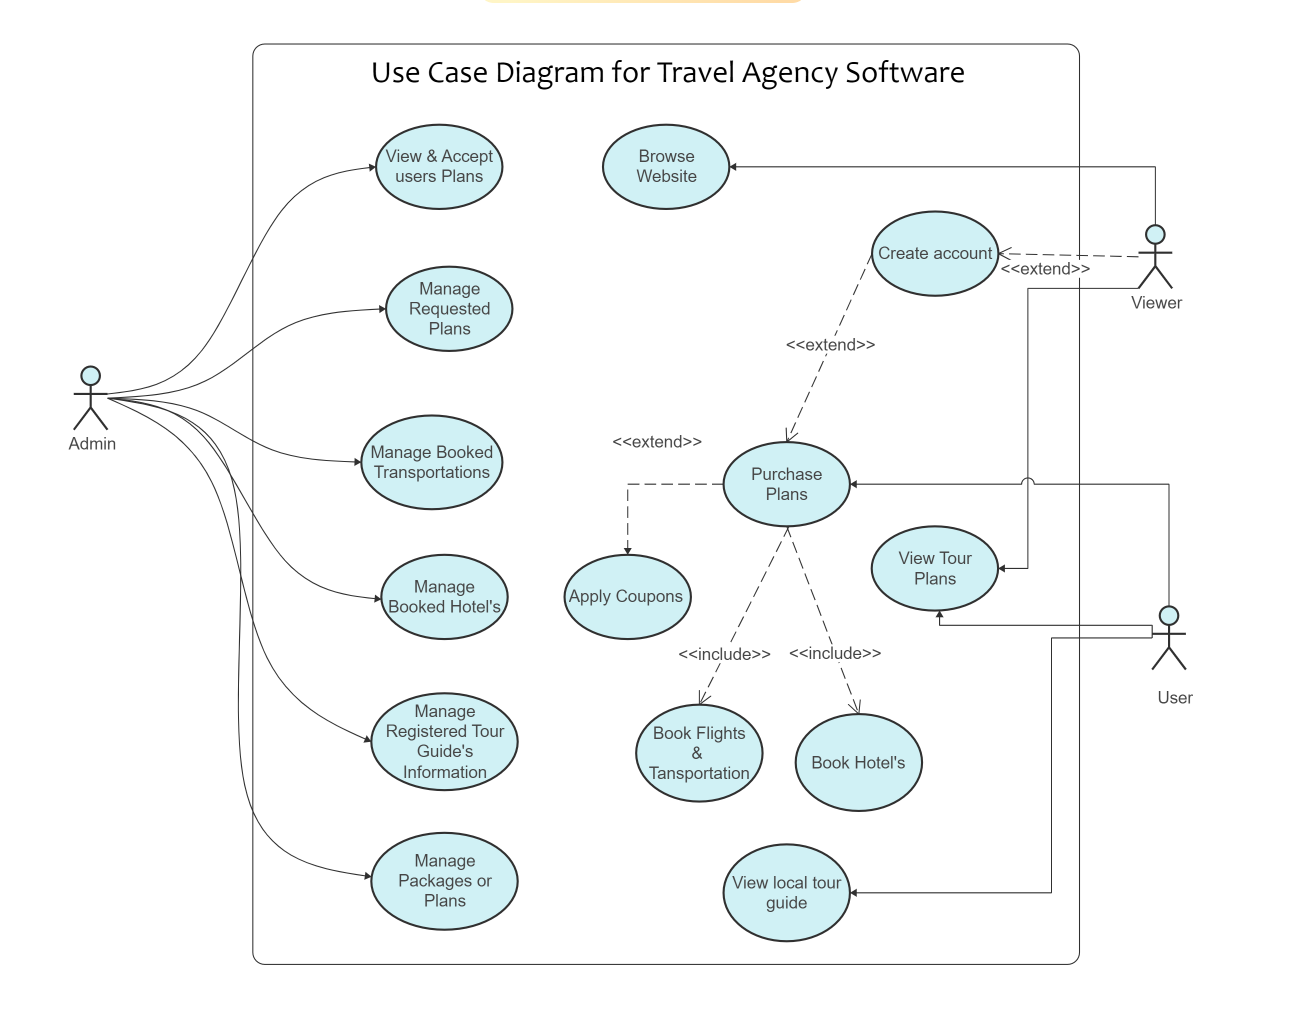
\includegraphics[width=450px, height=300px]{uml.png}}

\begin{center}
    \parbox{0.8\textwidth}{ 
        \centering
        \textbf{Figure - 7.9 : Use Case Diagram For Travel Agency Software}
    }
\end{center}

\section{ Sequence Diagram : }

The sequence diagram illustrates the interaction flow between a user and a travel booking system. It begins with the user browsing available travel packages. Upon selection of a package, the system prompts the user to either log in or register if not authenticated. The user provides their credentials or completes the registration process. The system verifies the provided information and authenticates the user. Once authenticated, the user confirms the booking details, including choosing transportation and accommodation options. The system processes the booking request and updates its database accordingly. Following successful booking, the system sends a confirmation message to the user, finalizing the transaction. Throughout this process, error handling mechanisms are in place to manage cases such as incorrect credentials or incomplete registrations. The sequence diagram effectively captures these interactions, detailing how information flows between the user and the system components involved in booking a travel package.

{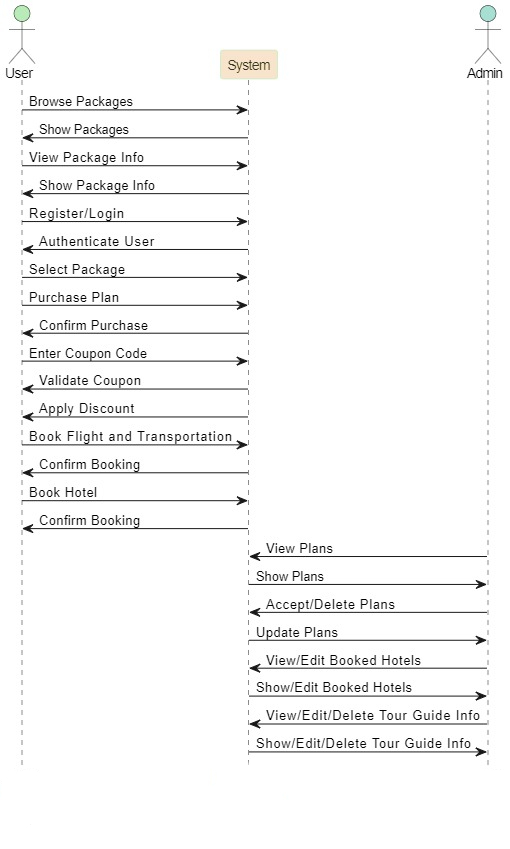
\includegraphics[width=450px, height=550px]{sqd.jpg}}

\begin{center}
    \parbox{0.8\textwidth}{ 
        \centering
        \textbf{Figure - 7.9 : Sequence Diagram For Travel Agency Software}
    }
\end{center}


\section{Data Flow Diagram}
DFD (Data Flow Diagram) helps us understand the how the data is flowing across the system and
what is the relation between the functions of the system.
Level 0 DFD and Level 1 DFD of Efficiency Monitor are shown in figure-9.1 and figure-9.2
respectively.





\section {Level-0 Data Flow Diagram}



\begin{center}
    \parbox{0.8\textwidth}{ 
        \centering
        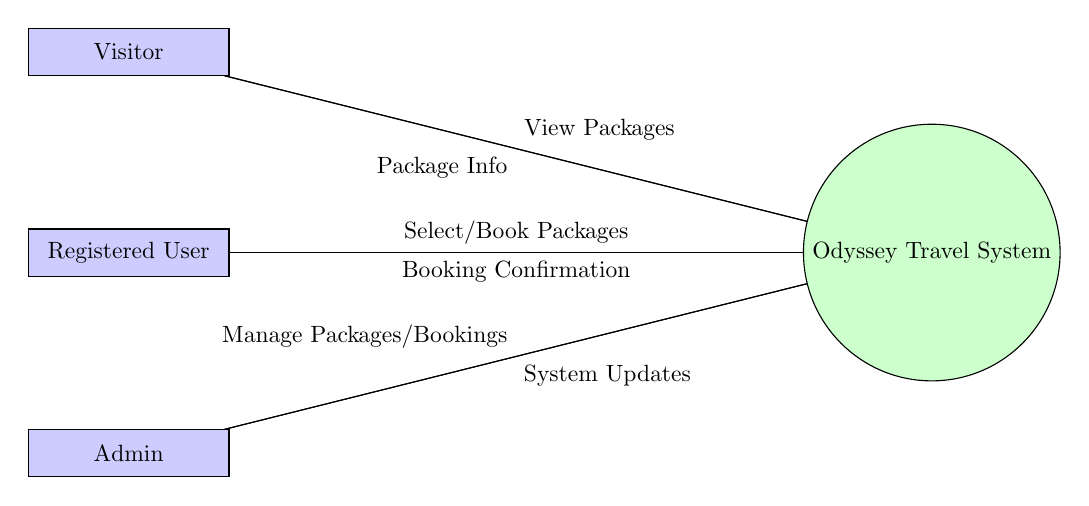
\begin{tikzpicture}[->,>=,auto,node distance=3cm,scale=0.85, transform shape]

            % Define styles
            \tikzstyle{external} = [rectangle, draw, fill=blue!20, text centered, minimum height=2em, minimum width=3cm]
            \tikzstyle{process} = [circle, draw, fill=green!20, text centered, minimum height=4em, minimum width=4em]
        
            % External Entities
            \node[external] (visitor) at (-6, 0) {Visitor};
            \node[external] (user) at (-6, -3) {Registered User};
            \node[external] (admin) at (-6, -6) {Admin};
        
            % Central Process
            \node[process] (system) at (6, -3) {Odyssey Travel System};
        
            % Data Flows
            \draw[->] (visitor) -- node[midway, midway] {View Packages} (system);
            \draw[->] (system) -- node[midway, midway] {Package Info} (visitor);
            \draw[->] (user) -- node[midway, midway] {Select/Book Packages} (system);
            \draw[->] (system) -- node[midway, below] {Booking Confirmation} (user);
            \draw[->] (admin) -- node[midway, midway] {Manage Packages/Bookings} (system);
            \draw[->] (system) -- node[midway, midway] {System Updates} (admin);
        
        \end{tikzpicture}
}
\end{center}

\begin{center}
    \parbox{0.8\textwidth}{ 
        \centering
        \textbf{Figure-9.1: Level 0 DFD of Travel Agency Software}
    }
\end{center}

\section{Level-1 Data Flow Diagram}

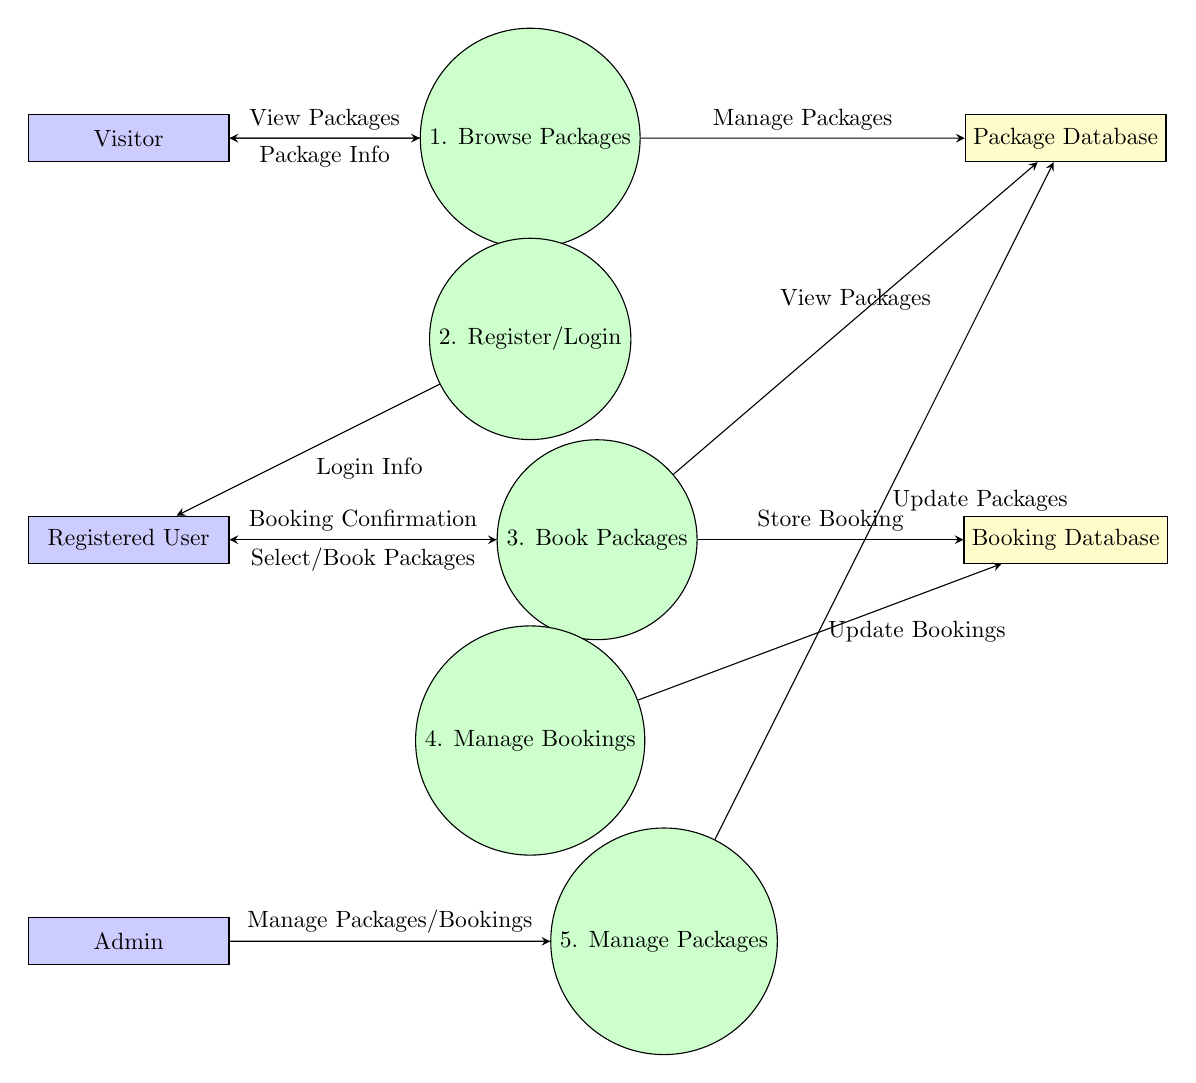
\begin{tikzpicture}[->,>=stealth,auto,node distance=4cm,scale=0.85, transform shape]

    % Define styles
    \tikzstyle{external} = [rectangle, draw, fill=blue!20, text centered, minimum height=2em, minimum width=3cm]
    \tikzstyle{process} = [circle, draw, fill=green!20, text centered, minimum height=4em, minimum width=4em]
    \tikzstyle{data} = [rectangle, draw, fill=yellow!20, text centered, minimum height=2em, minimum width=3cm]

    % External Entities
    \node[external] (visitor) at (-6, 6) {Visitor};
    \node[external] (user) at (-6, 0) {Registered User};
    \node[external] (admin) at (-6, -6) {Admin};

    % Data Stores
    \node[data] (packageDB) at (8, 6) {Package Database};
    \node[data] (bookingDB) at (8, 0) {Booking Database};

    % Processes with serial numbers
    \node[process] (browse) at (0, 6) {1. Browse Packages};
    \node[process] (register) at (0, 3) {2. Register/Login};
    \node[process] (book) at (1, 0) {3. Book Packages};
    \node[process] (manageBooking) at (0, -3) {4. Manage Bookings};
    \node[process] (managePackage) at (2, -6) {5. Manage Packages};

    % Data Flows
    \draw[->] (visitor) -- node[midway, above] {View Packages} (browse);
    \draw[->] (browse) -- node[midway, below] {Package Info} (visitor);
    \draw[->] (browse) -- node[midway, above] {Manage Packages} (packageDB);

    \draw[->] (user) -- node[midway, below] {Select/Book Packages} (book);
    \draw[->] (book) -- node[midway, above] {Booking Confirmation} (user);
    \draw[->] (book) -- node[midway, above] {Store Booking} (bookingDB);
    \draw[->] (book) -- node[midway, above] {View Packages} (packageDB);

    \draw[->] (admin) -- node[midway, above] {Manage Packages/Bookings} (managePackage);
    \draw[->] (managePackage) -- node[midway, right] {Update Packages} (packageDB);
    \draw[->] (manageBooking) -- node[midway, right] {Update Bookings} (bookingDB);

    \draw[->] (register) -- node[midway, midway] {Login Info} (user);

\end{tikzpicture}

\begin{center}
    \parbox{0.8\textwidth}{ 
        \centering
        \textbf{Figure-9.2: Level 1 DFD of Travel Agency Software}
    }
\end{center}


\section{ER Diagram}



\chapter{Conclussion}

In conclusion, the design of the Travel Agency Software presents a robust framework aimed at enhancing user experience and operational efficiency. By leveraging modern technologies such as Next.js for frontend development, Node.js for backend logic, and SQL databases for data management, the system ensures scalability and reliability. The integration of Tailwind CSS enhances the user interface, offering a responsive and visually appealing design. Authentication mechanisms using custom middleware and JWT tokens provide secure access control. The system's modular architecture facilitates easy maintenance and future enhancements, ensuring adaptability to evolving business needs. Overall, the Travel Agency Software is poised to streamline booking processes, optimize resource utilization, and deliver a seamless travel booking experience for users.

\end{document}